\documentclass[]{article}

\usepackage[T1]{fontenc}
\usepackage{textcomp}
\usepackage{amsmath, amssymb, amsthm}

\usepackage{tabularx}
\usepackage{setspace}
% figure support
\usepackage{import}
\usepackage{xifthen}
\usepackage{pdfpages}
\usepackage{transparent}
\usepackage{tabularx}

\title{Nuclear Waste Concern}
\date{Oct 03, 2022}
\author{Jack Ruder and Tatum Bunnett}


\begin{document}

\doublespacing
\maketitle

Dear Administrators of the Hanford Nuclear Facility, 
We are concerned community members worried about radiation exposures to ourselves along with our friends and families. 
Recently, we ran statistical tests to help analyze the relationship of radiation exposure and the amount of cancer deaths in 9 different counties. 
From the results of this statistical analysis we belive that our communites are entitiled to compensation. 
Below we express the reasons why we belive we deserve to be compensated, with statistical reasoning.
\section{Model and Analysis}
In examining data between Exposure and Cancer Mortality, a linear model was fit to the  data, as seen in Figure \ref{fig:ogdat}. The basic fit showed that the data is linear, though after experimentation, an even better fit was found using a square root transform of the Exposure data, seen in Figure \ref{fig:sqdat}. 
\begin{figure}[htpb]
	\centering
	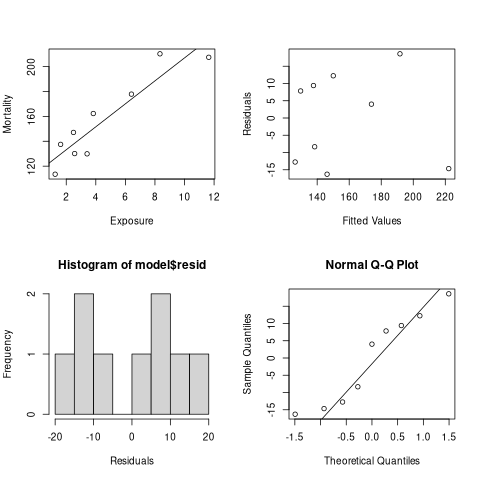
\includegraphics[width=0.6\textwidth]{"../originalData.png"}
	\caption{Linear fit on non-transformed data}
	\label{fig:ogdat}
\end{figure}
The fitted model is written as \begin{equation}M = 71.329 + 42.519 \cdot \sqrt{E}, \end{equation}
where \(M\) is the cancer mortality per 100000 man-years, and \(E\) is the index of exposure. Performing a t-test with this model gave a \(p\)-value for the slope of \(0.00017\), showing strong statistical significance of the model. We see an \(R^2\) of 0.88, confirming that Exposure and square-root Mortality are strongly correlated.  The baseline mortality here is 71.329, indicated by the intercept.

\begin{figure}[htpb]
	\centering
	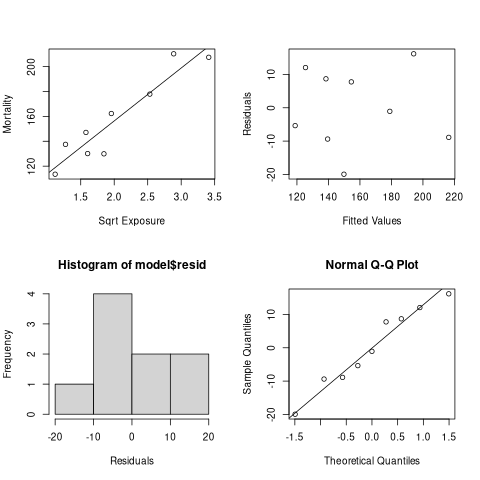
\includegraphics[width=0.6\textwidth]{"../sqrtExposreXmortality.png"}
	\caption{Linear fit on transformed data}
	\label{fig:sqdat}
\end{figure}
However, we still find a strong relationship in Exposure and Mortality, the fitted model without transforming Mortality had a p-value for the slope of 0.00033, and an \(R^2\) of 0.85. While the significance is not as strong, the linear model performs close enough to interperet meaning from its coefficients. The linear model is written as \begin{equation}M = 114.716 + 9.231 \cdot E.\end{equation} Thus, for every unit index of exposure, we see that an additional 9 out of every 100000 deaths will occur. A confidence interval shows that with 95\% of the time the slope will between 5.87 and 12.58. This is severe, with 12 units of exposure we would expect 1108 additional deaths over 10 years solely attributed to the exposure, assuming the mean slope of 9. Best case scenario would be seeing an additional 704 deaths, assuming a slope of 5.87. Neither of these scenarios are appropriate.

Using our square-root-transformed model, we may generate predictions of cancer mortality rates for low (<2), medium, and high (>5) exposures.

\begin{figure}[htpb]
	\centering
\begin{tabular}{r|c|c|c|c}
  & Pred. Lower & Pred. Upper & Conf. Lower & Conf. Upper \\
 \hline
 Low & 88.36 & 155.96 & 106.89 & 137.43 \\
 Med & 120.08 & 184.43 & 141.03 & 163.48  \\
 High & 169.70 & 240.81 & 186.57 & 223.94 \\
\end{tabular}
\end{figure}
We see that for low exposures, the lowest probable death rate is still higher than baseline (71.3 compared to 88.36). Freighteningly, the mortality could be as high as 155.96, doubling over no exposure.

\section{Concluding}
As you can see, damage to communities has been done with an increase in Mortality directly attributed to an increase in radioactive materials exposure. You should have also seen that there is still immense risk to low-exposure communities, and high-risk communities are even more in trouble. Please, consider these points as the damage is ongoing, reparations are needed urgently, especially in these high-exposure communities.
\end{document}
